\documentclass[a4paper, 11pt]{article}

%%% Packages
\usepackage[margin=50pt, vmargin={50pt, 10pt},includefoot]{geometry}
\usepackage{palatino}

%%% Listing package
\usepackage{listings}
\usepackage{color}
\usepackage{url}
\usepackage{hyperref}
\usepackage{setspace}
\usepackage{graphicx}
\DeclareGraphicsExtensions{.pdf,.png,.jpg}
\hypersetup{
  colorlinks = false,
  pdfborder={0 0 0}
}

\definecolor{dkgreen}{rgb}{0,0.6,0}
\definecolor{gray}{rgb}{0.5,0.5,0.5}
\definecolor{mauve}{rgb}{0.58,0,0.82}
\definecolor{red}{rgb}{0.8,0,0}
\definecolor{dkblue}{rgb}{0,0,0.6}

\lstset{ 
  language=C++,                  % the language of the code
  basicstyle=\footnotesize,       % the size of the fonts that are used for the code
  numbers=left,                   % where to put the line-numbers
  numberstyle=\tiny\color{gray},  % the style that is used for the line-numbers
  stepnumber=1,                   % the step between two line-numbers. If it's 1, each line 
  numbersep=5pt,                  % how far the line-numbers are from the code
  backgroundcolor=\color{white},      % choose the background color. You must add \usepackage{color}
  showspaces=false,               % show spaces adding particular underscores
  showstringspaces=false,         % underline spaces within strings
  showtabs=false,                 % show tabs within strings adding particular underscores
  frame=single,                   % adds a frame around the code
  rulecolor=\color{black},        % if not set, the frame-color 
  captionpos=b,                   % sets the caption-position to bottom
  breaklines=true,                % sets automatic line breaking
  breakatwhitespace=false,        %sets if automatic breaks should only happen at whitespace
  title=\lstname,                   % show the filename of files included with \lstinputlisting;
  keywordstyle=\color{blue},         % keyword style
  keywordstyle=[2]\color{dkgreen},
  commentstyle=\color{red},       %comment style
  keywords=[2]{vector, Action, State},
  stringstyle=\color{mauve},         %string literal style
  escapeinside={\%*}{*)},            % if you want to add LaTeX within your code
  emph={string, Puzzle, Board, multiset},  % emphasized characters
  emphstyle={\color{dkgreen}}
}

%%% End listing

%%%%%%%%%%%%%%%%%%%%%%%%%%%%%%%%%%%%%%%%%%%%%%%%%%%%%%%%%%%%%%%%%%%%%%%%%%%%%%%%%%%%%%%%%%%%%%%%%%%%%%%%%%%%%%%%%%%%%%%%%%%%%%%%%%%%%%%%%%%%%%%%%%%%%%%%%%%%%%%%%%%%%%%%%%%%%% 
\begin{document}
\begin{titlepage}
\title{\bf \Huge Jishu Pro Report\\
\huge AI's Pacman}
\author{By:\\ Le Trung Kien\\\\
03-120291\\
Department of Mechano-Informatics \\
The University of Tokyo
}
\maketitle
\thispagestyle{empty}
\end{titlepage}

%%%%%%%%%%%%%%%%%%%%%%%%%%%%%%%%%%%%%%%%%%%%%%%%%%
%%%%%%%%%%%%%%%%%%%%%%%%%%%%%%%%% Table of contents
\pdfbookmark[1]{Contents}{toc}  %%% additional bookmark for ToC
\tableofcontents
%%%%%%%%%%%%%%%%%%%%%%%%%%%%%%%%%%%%%%%%%%%%%%%%%%%%%%%%%%%%%%%%%%%%%%%%%%%%%%%%%%%%%%%%%%%%%%%%%%%%%%%%%%%%%%%%%%%%%%%%%%%%%%%%%%%%%%%%%%%%%%%%%%%%%%%%%%%%%%%%%%%%%%%%%%%%%% 

\newpage
\section{Pacman}

Pacman is classic game which was very popular in the 1980's. It is also a good benchmark to implement algorithms related to Artificial Intelligence and Machine Learning, especially good for testing adversarial search algorithms. The game I created here is a bit different from the original one due to the complexity of the game. Some notes about the game rules:
\begin{figure}[hbt]
  \centering
  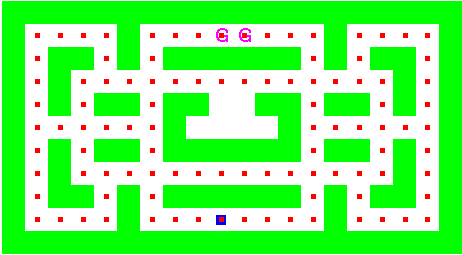
\includegraphics[width=4in]{field1-start}
  \caption[Close up of \textit{Hemidactylus} sp.]
  {Start field of Pacman game (G is ghost, Blue dot is Pacman)}
\end{figure}

\begin{itemize}
\item Size of the board: $9\times 18$ or larger.
\item There are two ghosts and one Pacman on the field.
\item Pacman wins when eating up foods.
\item Pacman looses when being eated by ghosts.
\item Ghosts cannot reverse directions, or stop.
\item The ghosts are normally in chasing mode but will turn to scared mode when Pacman eats speacial food known as power pellets.
\item Scared ghosts will return to normal after a specific number of moves.
\item After a ghost is eaten, a new ghost is born out of the center of the board.
\item Turn-taking game: Pacman first, then ghosts. Even though it looks like Pacman and Ghost simuntaneously make their moves, but in my implementation, pacman moves first, then ghosts choose their corresponding actions. This make the implementation simpler.
\end{itemize}
Normally, the task is to train Pacman to win the game, but I choose the opposition that is to make AI's ghosts. The two tasks have their own difficulty and appealing. 
\begin{itemize} 
\item AI's Pacman: Pacman wins only if he can eat all the foods without being eaten by ghosts. Therefore, when accessing a state from Pacman's point of view, we have to consider number of food left, distances from ghosts, distance to the nearest food.
\item AI's Ghosts: Ghosts, on the other hand, do not care about foods, so their only concern is to chase Pacman. However, ghosts are not alone, so this is a \textbf{collaborative task}, when two or more ghosts have to act together to win their game.
\end{itemize}
In short, the most interesting point of making AI's ghosts are their collaborative behaviour toward the same goal, kill Pacman.
\newpage
\section{Adversarial Search}
As the name suggests, adversarial search algorithms are in demand when adversary agents present. An agent cannot control its opponents or even its teammates' actions, that is why when making a move, it has to consider all possible outcomes of its and other agents' combined actions. The next following algorithms endevour to deal with a apecialized kind of games, which are deterministic, turn-taking.
\subsection{Minimax}
In Pacman game, Pacman is the Max player, while ghosts are Min players. The prototype for two main methods of MinimaxAgent class are: 
\begin{lstlisting}
virtual double Evaluate(const State &state, int depth, int player);
vector<Action> ChooseCombinedGhostAction(const State &state, int depth, double *v = NULL);
\end{lstlisting}
There is an ChoosePacmanAction method, but because my focus is to make AI's ghosts, so I will not present it here.
\begin{itemize}
\item \textbf{Evaluate State}: The state space of Pacman is very big, so we have to access a state even if it is not a terminal one. Basically, this function will define the efficiency of the algorithm. The better it evaluates a state, the stronger the chosen move will be.
\item \textbf{Choose Ghost Action}: After get all legal ghosts combined moves, those combinations are evaluated and the one that minimize the outcome is chosen. 
\end{itemize}
The mimimax algorithm performs a complete depth-first exploration of the game tree. If the maximum depth of the tree is m and there are b legal moves at each point, the the time complexity of the minimax algorithm is $\Theta (b^m)$. This is obviously infeasible for Pacman game, when b can be around 3, and m is very large. That is the reason why we need \textbf{Evaluate} method, instead of \textbf{Utility} method which only access the terminal state. The \textbf{depth} argument is used to limit the search space, that means, whenever the method reaches a terminal state or a state having the depth bound, it return a value.
\subsection{Alphabeta Pruning}
Alphabeta pruning is an enhanced version of Minimax algorithm in term of complexity. Therefore, AlphaBetaAgent class inherits almost all methods from MinimaxAgen class, except for the \textbf{Evaluation} method whose prototype is:
\begin{lstlisting}
double Evaluate(const State &state, int depth, int player, double alpha, double beta);
\end{lstlisting}
\begin{itemize}
\item Alpha is the highest value  we have found so far at any choice point along the path for MAX.
\item Beta is the lowest value we have found so far at any choise point along the path for MIN.
\end{itemize}
Alphabeta pruning algorithm produces the same results as Minimax does, but its complexity is $\Theta (b^{\frac{m}{2}})$, which is far better. We will see the difference in practice later in this report.
\subsection{Evaluation Function}
\subsection{Polynomial Combination}
Evaluation function is the one that decides Minimax or Alphabeta pruning algorithms' performance. Serveral features that I have tested are:
\begin{itemize}
\item{+} Pacman to ghosts Manhanttan distances: Ghosts want to minimize this distances
\item{-} Ghosts to ghosts Manhattan distances: Ghosts should not be too far and too close to each other. If they are separated, they will not be able to combine to kill Pacman. If they are too close, they become one Ghost and which is an advantage for Pacman.
\item{+} Pacman to ghosts graph distances:
\item{-} Ghosts to ghosts graph distances \\
  + means the bigger the better for MAX, while - means the smaller the better for MIN
\end{itemize}
At first, I used Manhattan distances as features and quickly recognized that they are not suitable for Pacman game because not every grids pair is connected. Therefore, I chose the latter two, which are the real distances between two grids. In order to do this, I used \textbf{A*} algorithm to calculate all the shortest between all possible pairs of grids in advanced. The interesting point is I was able to utilize the same Gsearch class I wrote for 8-15 puzzle in previous report. It emphasizes the reusablity of my code. \\
Many references suggest that the evaluating result should be a linear combination of features. However, by doing so, we also ignore all dependency among features. That is not a good idea. Finally, I came up with the following evaluation functions: 
\[ v = c_1*f_1+c_2*f_2+c_3*f_1*f_2\]
In which, $f_1$ is the total distance between Pacman and the two ghosts, and $f_2$ is the distance between two ghosts. Very few features here, but it turns out to be very powerful. The effect of this function will be discussed in the next section. \\
The actual implementation is:
\lstset{language=C++, caption={Evaluate method (utility.cpp)}}
\lstinputlisting[linerange={51-78}]{utility.cpp}
Because when Pacman is very close to Ghosts, the ghosts do not want to be next to each other. If they do so, they can not attack Pacman from different directions. Moreover, the two ghosts should never overlap each other too much. Therefore in those cases, I added an quite heavy weight to evaluation function. And when ghosts are far away from each other, I set it to Zero because at that point, all they should care is to get as close as possible to Pacman.

\subsection{Neural Network \& Optimization}
The above method of evaluating state, though, is reasonably good, has its litmitation. It is very hard to find good basic function to fully ultilize relationship among features. In classification task, we have exactly the same problem when using polynominal features to form features's space. Another way to evaluate a state is to use neural network. Because three layer neural network can approximate any function, we can evaluate any state through its features. Additionally, by using genetic algorithm, neural network can be trained to gain the optimal weights for accessing game's states. In order to do this, both backpropagatation neural network and genetic algorithm for mutating neural network were created. Pacman agent and Ghosts' agent compete against each other and theoretically they should both get better over time.

\section{Experiments}
Performance of this game depends on which algorithm is used and which evaluation's method is utilized. Comparison between minimax and alphabeta pruning with in term of complexity will be ilustrated as following. Numerous experiments are conducted to train the neural work with genetic algorithm. However, the results was not good enough compared with evaluation's function by polynomial combination of features. Therefore, only the latter will be mentioned here. 
\subsection{Execution} 
Please visit 
\begin{center}\textbf{\url{https://www.youtube.com/watch?v=9TLatwHJ27E}} \end{center}
to see numerous experiments I have done to test the algorithm with graphics user interface. I also asked some of my friends to play Pacman role, and they all easily lost to the Ghosts. Until now, I and my friends have not won a game against the Ghosts (algorithm = alphabeta pruning, depth = 14, coefficient=10,-5,5). Please give it a try if you have time, and if you win, please send the playing log to me. \\
Both GUI and CLI interfaces are provided. At any point of the game, if the Min value is $-1e6$ (INFINITY), the ghosts already know that they are going to win.
An example of running my application in command line. 
\begin{itemize}
\item To run the game
\begin{center} ./main algorithm depth $c_1$ $c_2$ $c_3$ \end{center}
\begin{table}[ht]
  \centering
  \begin{tabular}{|c|c|c|c|c|c|}
    \hline
    & algorithm & depth & $c_1$ & $c_2$ & $c_3$ \\ \hline
    description & minimax or alphabeta & depth bound&1st coeff & 2nd coeff &3rd coeff \\ \hline
    default & a & 12 & 10 & -5 & 5 \\
    \hline
  \end{tabular}
\end{table}
\item Press Up, Down, Left, Right arrow keys to move Pacman. Press Home to stop Pacman.
\item Press \textbf{'r'} to reset the game. 
\item Press \textbf{Esc} to end the game.

\end{itemize}
\begin{verbatim}
@:~/Dropbox/git/Pacman$ make
g++ -Wall -g -O2 -c -o state.o state.cpp
g++ -Wall -g -O2 -c -o common.o common.cpp
g++ -Wall -g -O2 -c -o minimaxAgent.o minimaxAgent.cpp
g++ -Wall -g -O2 -c -o utility.o utility.cpp
g++ -Wall -g -O2 -c -o alphabetaAgent.o alphabetaAgent.cpp
g++ -Wall -g -O2 -c -o main.o main.cpp
g++ -Wall -g -O2 -o main state.o common.o minimaxAgent.o utility.o alphabetaAgent.o main.o -lglut -lGL -lGLU
@:~/Dropbox/git/Pacman$ ./main a 12 10 -5 5
XXXXXXXXXXXXXXXXXXXX
X----X---GG---X----X
X-XX-X-XXXXXX-X-XX-X
X-X--------------X-X
X-X-XX-XX  XX-XX-X-X
X------X    X------X
X-X-XX-XXXXXX-XX-X-X
X-X--------------X-X
X-XX-X-XXXXXX-X-XX-X
X----X---P----X----X
XXXXXXXXXXXXXXXXXXXX
Number of food left: 100
Number of Evaluate: 10247
Minvalue: 250
Ghost Minimax Move: (L, R, )
XXXXXXXXXXXXXXXXXXXX
X----X--G--G--X----X
X-XX-X-XXXXXX-X-XX-X
X-X--------------X-X
X-X-XX-XX  XX-XX-X-X
X------X    X------X
X-X-XX-XXXXXX-XX-X-X
X-X--------------X-X
X-XX-X-XXXXXX-X-XX-X
X----X----P---X----X
XXXXXXXXXXXXXXXXXXXX
Number of food left: 99
.........................................................
Number of Evaluate: 1499
Minvalue: 70
Ghost Minimax Move: (L, L, )
XXXXXXXXXXXXXXXXXXXX
X----X--------X----X
X-XX-X-XXXXXX-X-XX-X
X-X---G----------X-X
X-X-XX-XX  XX-XX-X-X
X-----PX    X------X
X-X-XX XXXXXX-XX-X-X
X-X--- G      ---X-X
X-XX-X-XXXXXX X-XX-X
X----X----    X----X
XXXXXXXXXXXXXXXXXXXX
Number of food left: 85
Number of Evaluate: 2266
Minvalue: -1e+06
Ghost Minimax Move: (D, L, )
Pacman: LOSE
\end{verbatim}

\subsection{Minimax vs Alphabeta Pruning}
The following table shows comparision between Minimax and Alphabeta Pruning in term of number of evaluated nodes. The depth is set as 12.
\begin{table}[ht]
  \centering
  \begin{tabular}{|c|c|r|r|}
    \hline
    Pacman Move & Ghost Moves & Minimax & Alphabeta Pruning \\ \hline
    r           & l,r         & 5824    & 1936              \\ \hline
    r           & l,r         & 5299    & 1554              \\ \hline
    r           & l,r         & 10514   & 1478              \\ \hline
    r           & d,d         & 22021   & 2182              \\ \hline
    u           & d,d         & 61080   & 1855              \\ \hline
    u           & r,d         & 286179  & 20064             \\ \hline
    r           & r,d         & 49025   & 1119              \\ \hline
    r           & r,d         & 109956  & 3288              \\ \hline
    r           & r,d         & 66916   & 5059              \\ \hline
    u           & r,r         & 66804   & 9269              \\ \hline 
    u           & r,r         & 17848   & 2193              \\ \hline
    l           & r,r         & 13621   & 1660              \\ \hline
    l           & d,u         & 17056   & 1673              \\ 
    \hline
  \end{tabular}
\end{table}
Clearly Alphabeta pruning is much more efficient than Minimax. Notice that number of evaluated nodes varies a lot due to the different number of legal moves. Alphabeta pruning performance also depends on the order of examined nodes. The sooner the best move is found, the more nodes can be pruned. 

\section{Game State}
The State class, which represents the Game state take me lots of hours to complete. It was hard to think from how to represent the game state to how to make transition from a state to another. The class declaration is shown in the following Listing.
\lstset{language=C++, caption={state class (state.hpp)}}
\lstinputlisting[linerange={10-68}]{state.hpp}
Please refer to the source code \textbf{state.cpp} for more details about this class. 
\section{Discussion}
Firstly, I want to talk about the Evaluation function. As mentioned above, this function is the most important aspect of Minimax and Alphabeta pruning algorithm. In a limited time, I think I considered a very simple version of it. In order to optimize the Evaluation function, we can add more features to it, and try to combine features in more sophisticated way such as Neural Network. I think it is possible to combine Neural Network and Genetic Algorithm to find the optimal evaluation function to this problem. That is maybe the theme for my next report. \\
Secondly, Alphabeta pruning is much more efficient than Minimax algorithm. In real applications, probably minimax will never be used. The game now is a deterministic one, however, if uncertainty is taken into account, we have an other algorithm called Expectimax. In this case, opponents do not always take their best moves, they sometimes take other moves which produce different outcomes. \\
Finally, I admit I regret not to make hardware for Jishu Pro, since it was probably the last chance for me to touch hardware. I am seriously interested in Artificial Intelligence and Machine Learning, so I decided to use Pacman as a platform to implement those algorithms I have learned. However, there would have been much more fun if I had made some hardware, such as a Pacman and a ghost fighting against each other. 

\begin{thebibliography}{9}
\bibitem{AIMA}
  \label{itm:AIMA}
  Stuart Russell, Peter Norvig
  \emph{  Aritifical Intelligence A Modern Approach},
  Prentice Hall
  3rd Edition,
  December 2009

\bibitem{SSCPS}
  \label{itm:SSCPS}
  George F. Luger
  \emph{Artificial Intelligence, Structure and Strategies for Complex Problem Solving},
  Addison Wesley Longman
  3rd Edition,
  2009
  
\bibitem{Algorithms}
  \label{itm:algorithm}
  Robert Sedgewick, Kevein Wayne
  \emph{ Algorithms}
  Addison Wesley
  4th Edition,
  January, 2012

\bibitem{PRML}
  \label{itm:PRML}
  Christopher M. Bishop
  \emph{Pattern Recognition and Machine Learning},
  Springer
  1st Edition,
  2006
  
\end{thebibliography}
\end{document}
%%%%%%%%%%%%%%%%%%%%%%%%%%%%%%%%%%%%%%%%%%%%%%%%%%%%%%%%%%%%%%%%%%%%%%%%%%%%%%%%%%%%%%%%%%%%%%%%%%%%%%%%%%%%%%%%%%%%%%%%%%%%%%%%%%%%%%%%%%%%%%%%%%%%%%%%%%%%%%%%%%%%%%%%%%%%%% 